\chapter{Order and lattices}\label{ch:order}

In this chapter we first introduce basic notions from order theory: preorders, partial orders, and lattices. We then zoom in on distributive lattices. In the finite case, we prove from first principles a duality theorem, which is a blueprint for the more advanced duality theorems that follow later in this text.\endnote{We recommend \cite{DavPri2002} for a more detailed introduction to order and lattice theory. In addition, the classic \cite{BalDwi1974} remains a good resource for the basics of lattice theory, although it is somewhat outdated when it comes to the more advanced theory.}\astfootnote{The numbered notes can be found at the end of each chapter.}

\section{Preorders, partial orders, suprema and infima}\label{sec:orders}
A binary relation $\preceq$ on a set $P$ is called
\begin{itemize}
\item \emph{reflexive} if $p \preceq p$ for all $p \in P$,
\item \emph{transitive} if $p \preceq q \preceq r$ implies $p \preceq r$ for all $p,q,r \in P$,
\item \emph{anti-symmetric} if $p \preceq q$ and $q \preceq p$ imply $p = q$ for all $p, q \in P$,
\item a \emph{preorder} if it is reflexive and transitive,
\item a \emphind{partial order} if it is reflexive, transitive and anti-symmetric.
\end{itemize}
A \emph{preordered set}\index{preorder} is a tuple $(P,\preceq)$ with $\preceq$ a preorder on the set $P$. A \emphind{poset}\index{partial order} (short for partially ordered set) is a pair $(P,\leq)$ with $\leq$ a partial order on the set $P$.

Two elements $p$ and $q$ are \emphind{comparable} in a preorder $\preceq$ if at least one of $p \preceq q$ and $q \preceq p$ holds, and \emphind{incomparable} otherwise. The adjective `partial' in `partial order' refers to the fact that not all elements in a partial order are comparable.

A preorder is called \emph{total} or \emph{linear} if any two of its elements are comparable.
A \emphind{total order} or \emphind{linear order} or \emphind{chain} is a total preorder which is moreover anti-symmetric. A poset is called an \emphind{anti-chain} if no distinct elements are comparable.

The \emphind{strict part} of a partial order is the relation $<$ defined by $p < q$ if, and only if, $p \leq q$ and $p \neq q$. Notice that to specify a partial order $\leq$, it suffices to specify its strict part $<$, from which we can then define $p \leq q$ if, and only if, $p < q$ or $p = q$.

\begin{example} \index{diamond poset} \index{Boolean algebra on 2 atoms}
  In Figure~\ref{fig:diamond}, we draw the so-called \emph{Hasse diagram} of the `diamond' poset $D = \{a,b,c,d\}$, with partial order ${\leq}$ whose strict part is $\{(a,b),(a,c),(a,d),(b,d),(c,d)\}.$
  This partial order is not linear, because we have neither $b \leq c$ nor $c \leq b$.

  \begin{figure}
  \begin{center}
  \begin{tikzpicture}
  \polab{(0,0)}{$b$}{left}
  \polab{(1,-1)}{$a$}{below}
  \polab{(1,1)}{$d$}{above}
  \polab{(2,0)}{$c$}{right}
  \li{(0,0)}{(1,-1)}
  \li{(0,0)}{(1,1)}
  \li{(1,-1)}{(2,0)}
  \li{(1,1)}{(2,0)}
  \end{tikzpicture}
  \end{center}
  \vspace{-5mm}
  \caption{The `diamond' poset $(D,\leq)$}
  \label{fig:diamond}
  \end{figure}

\end{example}
Notice that, in the above example, even though $a \leq d$, we did not draw an edge between $a$ and $d$ in the Hasse diagram. This is due to the fact that $a \leq d$ can be inferred by transitivity from the order relations $a \leq b$ and $b \leq d$, which are depicted in the diagram. Thus, we only need to draw the `covering' relations in the diagram.

We now give the general definition of \emph{Hasse diagram}. For elements $p$, $q$ of a poset $P$, we say that $q$ \emph{covers} $p$ if $p < q$ and there is no $r$ such that $p < r < q$. The elements of a poset are represented in the Hasse diagram as nodes, with the convention that moving up along an edge in the diagram corresponds to moving up in the order, while points drawn at the same height are incomparable. An edge is drawn from a node $p$ to a node $q$ whenever $q$ covers $p$.

There are several interesting classes of maps between preordered sets.
Let $(P,\preceq_P)$ and $(Q,\preceq_Q)$ be preordered sets and $f \colon P \to Q$ a function. The function $f$ is called
\begin{itemize}
\item \emphind{order preserving} if $p \preceq_P p'$ implies $f(p) \preceq_Q f(p')$ for all $p, p' \in P$,
\item \emphind{order reflecting} if $f(p) \preceq_Q f(p')$ implies $p \preceq p'$ for all $p, p' \in P$,
\item an \emphind{order-embedding} if it is both order preserving and order reflecting,
\item an \emphind{order-isomorphism} if it is order preserving and has an order preserving inverse.
\end{itemize}
Note that order-embeddings between posets are always injective, but not all injective order-preserving maps between posets are order-embeddings! (Exercise~\ref{exe:orderemb}\ref{exe:injnotemb}.) A function $f$ between preordered sets is an order-isomorphism if and only if $f$ is a surjective order-embedding (Exercise~\ref{exe:orderemb}\ref{exe:surjembisiso}).

An elementary but important operation on preorders is that of `turning upside down'. If $P$ is a preorder, we denote by $P^\mathrm{op}$\nomenclature[opposite]{$()^{\mathrm{op}}$}{opposite} the \emphind{opposite} of $P$, i.e., the preorder with the same underlying set as $P$, but with preorder $\preceq'$ defined by $p \preceq' q$ if, and only if, $q \preceq p$, where $\preceq$ denotes the original preorder on $P$.










\begin{example} \label{exa:finitetotal}
For any natural number $n$, the finite set $\mathbf{n} := \{0,1,\dots,n-1\}$\nomenclature[n-element]{$\mathbf{n}$}{$n$-element lattice} is totally ordered by the usual ordering of natural numbers. %
\end{example}

\begin{example} \label{exa:totalorders}
The sets of natural numbers $\mathbb{N}$, integers $\mathbb{Z}$, rational numbers $\mathbb{Q}$, and real numbers $\mathbb{R}$, with the usual orders, are total orders. %
\end{example}

\begin{example} \label{exa:preordernaturals}
On the set of natural numbers $\mathbb{N}$, define a relation $\preceq$ by
\[ p \preceq q \iff p = 0 \text{ or } (p \neq 0 \text{ and } q \neq 0).\]
Note that $\preceq$ is a preorder, but not a partial order. Consider the quotient of $\mathbb{N}$ by the equivalence relation that identifies all non-zero numbers.
This is a poset, and it is in fact the largest poset quotient of the preorder $(\mathbb{N},\preceq)$. Such a quotient always exists and is called the \emphind{poset reflection} of the preorder; see Exercise~\ref{exe:reflection}.
\end{example}



\begin{example}\label{exa:logicequivalence}
Let $F$ be a set of formulas in some logic with a relation of derivability $\vdash$ between formulas of $F$. More concretely, $F$ can be the set of sentences in a first-order signature and $\vdash$ derivability with respect to some first-order theory. The proof rules `identity' and `cut' state precisely that $\vdash$ is a preorder on $F$. The relation $\vdash$ is rarely a partial order, as there are usually many syntactically different formulas which are inter-derivable in the logic. The poset reflection (Exercise~\ref{exe:reflection}) consists of the $\vdash$-equivalence classes of formulas in $F$.
\end{example}

\begin{example} \label{exa:sequenceorders}
Denote by $\mathbf{2}^*$ the set of finite sequences over the two-element set $\mathbf{2} = \{0,1\}$.
\begin{enumerate}
\item For $p, q \in \mathbf{2}^*$, define
\[ p \leq_P q \iff \text{ there exists } r \in \mathbf{2}^* \text{ such that } pr = q.\]
Note that $\leq_P$ is a partial order on $\mathbf{2}^*$, see Exercise~\ref{exe:prefixorder} below. The poset $(\mathbf{2}^*,\leq_P)$ is called the \emphind{full infinite binary tree}. %
The partial order $\leq_P$ on $\mathbf{2}^*$ is called the \emphind{prefix order}.\label{exa:binaryprefix}
\item For $p = (p_1,\dots,p_n)$ and $q = (q_1,\dots,q_n) \in \mathbf{2}^*$, define $p \leq_L q$ if, and only if, $p \leq_P q$, or $p$ and $q$ have the same length and $p_i \leq q_i$, where $1 \leq i \leq n$ is the least index such that $p_i \neq q_i$.
Note that $\leq_L$ is a partial order on $\mathbf{2}^*$ (see Exercise~\ref{exe:lexico} below). The partial order $\leq_L$ is called the \emph{lexicographic}\index{lexicographic order} or \emphind{dictionary order} on $\mathbf{2}^*$.\label{exa:binarylexico}
\end{enumerate}
\end{example}









We define the fundamental notions of supremum and infimum.

\begin{definition}\label{def:supinf}
Let $(P,\preceq)$ be a preorder. Let $S \subseteq P$.
\begin{itemize}
\item an element $s_0$ of $P$ is called a \emphind{lower bound} of $S$ if $s_0 \preceq s$ for all $s \in S$;
\item an element $s_1$ of $P$ is called an \emphind{upper bound} of $S$ if $s \preceq s_1$ for all $s \in S$;
\item a lower bound $s_0$ of $S$ is called an \emphind{infimum} or \emphind{greatest lower bound} of $S$ if, for any lower bound $s'$ of $S$, $s' \preceq s_0$;
\item an upper bound $s_1$ of $S$ is called a \emphind{supremum} or \emphind{least upper bound} of $S$ if, for any upper bound $s'$ of $S$, $s_1 \preceq s'$.
\end{itemize}
In the special case where $S = \emptyset$, an element $s_0$ which is a supremum of $S$ is called a \emphind{bottom} or \emph{least} element of $P$, and an element $s_1$ which is an infimum of $S$ is called a \emphind{top} or \emph{greatest} element of $P$.
\end{definition}
In a poset, any set has at most one infimum and at most one supremum (Exercise~\ref{exe:infsupunique}). If a unique infimum of a subset $S$ exists, it is denoted by $\bigwedge S$\nomenclature{$\bigwedge$}{meet} and is also known as the \emphind{meet} of $S$. The supremum of $S$, if it exists uniquely, is denoted by $\bigvee S$ and is known as the \emphind{join}\nomenclature{$\bigvee$}{join} of $S$. In the case where $S = \{a,b\}$, we also write $a \wedge b$ and $a \vee b$, and if $S = \{a_1,\dots,a_n\}$ we write $a_1 \vee \cdots \vee a_n$ and $a_1 \wedge \cdots \wedge a_n$. The bottom element, if it exists, is denoted by $\bot$\nomenclature{$\bot$}{bottom} or $0$, and the top element by $\top$\nomenclature{$\top$}{top} or $1$.

\begin{remark}\index{maximal vs. maximum}\index{supremum!vs. maximum}
There are subtle but important differences between the words `maximum', `maximal' and `supremum'. An element is \emph{maximal} in a subset $S$ of a poset if there is no other element in $S$ that lies strictly above it, while it is a \emph{maximum} element in $S$ if all other elements of $S$ lie below it. Note that in a \emph{totally} ordered set, the concepts maximal and maximum are equivalent, but not in general. Finally, an important distinction between these two concepts and that of supremum is that for an element to be a supremum, it is \emph{not} needed that it lies in the set itself, while this is part of the definition for maximal and maximum elements. See Exercise~\ref{exe:umalsup}.
\end{remark} %

Infima and suprema may fail to exist. There are two reasons why this can happen: a set can either have no lower (or upper) bounds at all, or its set of lower (or upper) bounds has incomparable maximal (or minimal) elements.

We illustrate the above ideas with three examples.
\begin{example}\label{exa:butterfly}
In the poset $(P,\leq)$ whose Hasse diagram is depicted below, the set $S = \{a,b\}$ does not have an infimum, because $c$ and $d$ are incomparable maxim\emph{al} lower bounds of $S$, and hence neither is a maxim\emph{um} lower bound.
\index{butterfly poset}


\begin{figure}[htp]
\begin{center}
\begin{tikzpicture}
\polab{(0,1)}{$a$}{left}
\polab{(1,1)}{$b$}{right}
\polab{(0,0)}{$c$}{left}
\polab{(1,0)}{$d$}{right}
\li{(0,0)}{(0,1)}
\li{(0,0)}{(1,1)}
\li{(1,0)}{(0,1)}
\li{(1,0)}{(1,1)}
\end{tikzpicture}
\end{center}
\vspace{-5mm}
\caption{The `butterfly' poset $(P,\leq)$}
\label{fig:butterfly}
\end{figure}
\end{example}

\begin{example}\label{exa:naturalsinfsup}
In the set $\mathbb{N}$ of natural numbers with its usual total order, any subset has an infimum, which is in fact a minimum, but the only subsets having a supremum are the finite subsets. For any finite subset, the supremum is in fact a maximum.
\end{example}

\begin{example}\label{exa:rationalsinf}
In the set $\mathbb{Q}$ of rational numbers with its usual total order, the subset $\{\frac{1}{n} \ | \ n \in \mathbb{N}_{\geq 1}\}$ has an infimum, $0$, but it does not have a minimum.
\end{example}

We end this section by introducing the important concepts of \emph{adjunction} and \emph{Galois connection} between preordered sets.\index{adjunction!between preorders} 
\begin{definition}\label{dfn:poset-adjunction-def}
  Let $(P,\preceq_P)$ and $(Q,\preceq_Q)$ be preordered sets, and let $f \colon P \to Q$ and $g \colon Q \to P$ be order-preserving functions. The pair $(f,g)$ is called an \emph{adjunction}, with $f$ the \emph{left} or \emph{lower adjoint} and $g$ the \emph{right} or \emph{upper adjoint}, if, for every $p \in P$ and $q \in Q$,\index{adjoint!between preorders}
\[ f(p) \preceq_Q q \text{ if, and only if, } p \preceq_P g(q).\]
An adjunction between $P^\op$ and $Q$ is called a \emphind{Galois connection} or \emphind{contravariant adjunction}.
\end{definition}
The notion of adjunction between preorders is a special case of the concept of adjunction between categories that we will encounter later, see Chapter~\ref{ch:categories}, p.~\ref{dfn:adjunction}. The concept of a (contravariant) adjunction between preorders will already play a role earlier, in Section~\ref{sec:quotients-and-subs}, when we study connections between sublattices and quotient spaces, analogous to the original connection studied by Galois, which was between subgroups and field extensions. Exercises~\ref{exe:adjunctions}~and~\ref{exe:adjointexistsiff} below collect some basic important facts about adjunctions between pre-orders, which will be used throughout the book.

\begin{example}
  Let $f \colon \mathbb{Z} \into \mathbb{Q}$ be the order-embedding which sends each integer $x \in \mathbb{Z}$ to itself, regarded as a rational number. The map $f$ has a right adjoint, $g$, which sends each rational $y \in \mathbb{Q}$ to its \emph{floor}, i.e., $g(y)$ is the largest integer below $y$. The map $f$ also has a left adjoint, which sends a rational $y \in \mathbb{Q}$ to its \emph{ceiling}, i.e., the smallest integer above $y$.
\end{example}
\begin{example}\label{exa:galoisconnection}
  Fix a relation $R \subseteq X \times Y$ between two sets. For any $a \subseteq X$ and $b \subseteq Y$, define the sets $u(a) \subseteq Y$ and $\ell(b) \subseteq X$ by
  \begin{align*}
    u(a) &:= \{y \in Y \ \colon \ \text{for all } x \in a, x {R} y \}, \\
  \ell(b) &:= \{ x \in X \ \colon \ \text{for all } y \in b, x {R} y \}
  \end{align*}
  The pair of functions $u \colon \mathcal{P}(X) \leftrightarrows \mathcal{P}(Y) \colon \ell$ is a Galois connection between the posets $(\mathcal{P}(X), \subseteq)$ and $(\mathcal{P}(Y), \subseteq)$, i.e., for any $a \subseteq X$ and $b \subseteq Y$, we have $b \subseteq u(a)$ if, and only if, $a \subseteq \ell(b)$.
\end{example}
  We mention two well-known special cases of the Galois connection of Example~\ref{exa:galoisconnection}.
  
  First, in the special case when $R$ is a pre-order on a set $X$, $u(a)$ is the set of \emph{common upper bounds} for the elements of $a$, and $\ell(b)$ is the set of \emph{common lower bounds} for the elements of $b$.

  Second, the Galois connection between theories and model classes from logic is also a special case of the Galois connection $(u,\ell)$, as follows. Suppose that $S$ is a set of structures, $F$ is a set of logical formulas, and suppose we are given a relation of `interpretation', $\models$ from $S$ to $F$, where, for $M \in S$ and $\phi \in F$, the relation $M \models \phi$ is read as ``$\phi$ holds in $M$''. Then in the above Galois connection, $u$ sends a set of models $a$ to its \emph{theory}, i.e., the set of formulas that hold in every model of $a$, and $\ell$ sends a set of formulas $b$ to its \emph{class of models}, i.e., the set of models in which every formula from $b$ holds.





\exercises


\begin{exercise}\label{exe:hasse}
Sketch the Hasse diagrams for the preorders described in Example~\ref{exa:finitetotal}, Example~\ref{exa:preordernaturals} and Example~\ref{exa:sequenceorders}(\ref{exa:binaryprefix}).

\end{exercise}

\begin{exercise}\label{exe:prefixorder}\index{free monoid}
For any set $A$, let $A^*$ denote the set of finite sequences of elements of $A$. Prove that the relation $\leq_P$ on $A^*$ defined by
\[ u \leq_P v \iff \text{ there exists } w \text{ such that } uw = v\]
is a partial order.

{\it Remark.} This is a special case of the opposite of the so-called Green pre-order $\leq_{\mathcal{R}}$, which exists on any monoid.
\end{exercise}

\begin{exercise}\label{exe:lexico}\index{lexicographic order}
Consider the relation $\leq_L$ on $\mathbf{2}^*$ defined in Example~\ref{exa:sequenceorders}\ref{exa:binarylexico}.
\begin{enumerate}
\item Prove that $\leq_L$ is a partial order which is not total.
\item Sketch the Hasse diagram of $(\mathbf{2}^*,\leq_L)$.
\end{enumerate}
\end{exercise}

\begin{exercise}\label{exe:orderemb}
\begin{enumerate}
\item Give an example of an injective order-preserving map between posets which is not an order-embedding.\label{exe:injnotemb}\index{order-preserving!and injective}
\item Prove that a surjective order-embedding between posets is an order-isomorphism.\label{exe:surjembisiso}\index{order-embedding!surjective}
\end{enumerate}
\end{exercise}



\begin{exercise}\label{exe:reflection}
If $(P,\preceq)$ is a preordered set, define
\[ p \equiv q \iff p \preceq q \text{ and } q \preceq p.\]
If $p \equiv q$, we say $p$ and $q$ are \emph{equivalent}.
\begin{enumerate}
\item Prove that $\equiv$ is an equivalence relation on $P$.
\item Prove that there is a well-defined \emph{smallest} partial order $\leq$ on the quotient set $P/{\equiv}$ such that the quotient map $f \colon P \to P/{\equiv}$ is order preserving.
\item Prove that, for any order-preserving $g \colon P \to Q$ with $Q$ partially ordered, there exists a unique order-preserving $\overline{g} \colon P/{\equiv} \to Q$ such that $\overline{g} \circ f = g$.
\end{enumerate}
The partial order $P/{\equiv}$ defined in this exercise is called the \emphind{poset reflection} of the preorder $P$.
\end{exercise}




\begin{exercise}\label{exe:infsupunique}
Let $(P,\preceq)$ be a preorder and $S \subseteq P$.
\begin{enumerate}
\item Prove that if $s_0$ and $s_0'$ are both infima of $S$, then $s_0 \preceq s_0'$ and $s_0' \preceq s_0$.
\item Conclude that in a partial order, any set has at most one supremum and at most one infimum.
\end{enumerate}
\end{exercise}
\begin{exercise}\label{exe:umalsup}
Draw a graph with three nodes labelled `maximum', `maximal', and `supremum', and directed edges denoting that the existence of one implies the existence of the other. Do any more implications hold in finite posets? In totally ordered sets? In finite totally ordered sets?
\end{exercise}

\begin{exercise}\label{exe:adjunctions}
  Let $(P,\preceq_P)$ and $(Q,\preceq_Q)$ be preordered sets and $f \colon P \leftrightarrows Q \colon g$ a pair of order-preserving maps between them.
  \begin{enumerate}
  \item Prove that $(f,g)$ is an adjunction if, and only if, for every $p \in P$, $p \preceq_P gf(p)$, and for every $q \in Q$, $fg(q) \preceq_Q q$.
  \end{enumerate}
  Now assume that $(f,g)$ is an adjunction.
  \begin{enumerate}[resume]
  \item Prove that $fgf(p) \equiv f(p)$ and $gfg(q) \equiv g(q)$ for every $p \in P$ and $q \in Q$.
  \item Conclude that, in particular, if $P$ and $Q$ are posets, then $fgf = f$ and $gfg = g$.
  \item \label{itm:minimumimage} Prove that, if $P$ is a poset, then for any $p \in P$, $gf(p) = \min (\mathrm{im}(g) \cap {\uparrow} p)$, i.e., $gf(p)$ is the minimum element above $p$ that lies in the image of $g$.
  \item Formulate and prove a similar statement to the previous item about $fg(q)$, for $q \in Q$.
  \item \label{itm:leftadjointpreservessup} Prove that, for any subset $S \subseteq P$, if the supremum of $S$ exists, then $f\left(\bigvee S\right)$ is the supremum of $f(S)$.
  \item Prove that, for any subset $T \subseteq Q$, if the infimum of $T$ exists, then $g\left(\bigwedge T\right)$ is the infimum of $g(T)$.
  \end{enumerate}
  In words, the last two items say that \emph{lower adjoints preserve existing suprema} and \emph{upper adjoints preserve existing infima}. In Exercise~\ref{exe:adjointexistsiff} of the next section we will see that a converse to this statement holds in the context of complete lattices.
  \end{exercise}

\section{Lattices}\label{sec:lattices}
A \emph{(bounded) lattice}\index{lattice!order-theoretic definition} is a partially ordered set $L$ in which every finite subset has a supremum and an infimum.  In fact, to be a lattice, it is sufficient that the empty set and all two-element sets have suprema and infima, see Exercise~\ref{exe:lattsuff}. A \emphind{complete lattice} $C$ is a partially ordered set in which every subset has a supremum and an infimum. In fact, for a partially ordered set to be a complete lattice, it is sufficent that every subset has a supremum, see Exercise~\ref{exe:complattsuff}.\endnotemark
\endnotetext{Lattices, according to our definition, in particular always have a top and a bottom element. Some authors use a different definition, and define a lattice to be a poset in which suprema and infima of \emph{non-empty} finite subsets exist. These authors then say a lattice is \emph{bounded}\index{lattice!bounded} if it moreover has a top and bottom. Since almost all lattices we consider have top and bottom elements, we include this in the definition, and we take care to say so explicitly if top and bottom elements fail to exist.}

An interesting equivalent definition of lattices is the following. A \emph{lattice}\index{lattice!algebraic definition} is a tuple $(L,\vee,\wedge,\bot,\top)$, where $\vee$ and $\wedge$ are binary operations on $L$ (i.e., functions $L \times L \to L$), and $\bot$ and $\top$ are elements of $L$ such that the following axioms hold:
\begin{enumerate}
\item the operations $\vee$ and $\wedge$ are \emphind{commutative}, i.e., ${a \vee b = b \vee a}$ and \newline${a \wedge b = b \wedge a}$ for all $a, b \in L$;
\item the operations $\vee$ and $\wedge$ are \emphind{associative}, i.e., ${(a \vee b) \vee c = a \vee (b \vee c)}$ and ${(a \wedge b) \wedge c = a \wedge (b \wedge c)}$ for all $a, b, c \in L$;
\item the operations $\vee$ and $\wedge$ are \emphind{idempotent}, i.e., $a \vee a = a$ and $a \wedge a = a$ for all $a \in L$;
\item the \emphind{absorption laws} $a \wedge (a \vee b) = a$ and $a \vee (a \wedge b) = a$ hold for all $a, b \in L$;
\item the element $\bot$ is \emph{absorbing for $\wedge$} and the element $\top$ is \emph{absorbing for~$\vee$}, i.e., $\bot \wedge a = \bot$ and $\top \vee a = \top$ for all $a \in L$.%
\end{enumerate}
Given a lattice~$(L,\vee,\wedge,\bot,\top)$ according to this algebraic definition, define
\[ a \leq_L b \iff a \wedge b = a.\]
Then $\leq_L$ defines a partial order on the set $L$ which makes $L$ into a lattice according to the order-theoretic definition. Conversely, given a lattice~${(L,\leq)}$ according to the order-theoretic definition, it is easy to check that the operations of binary join ($\vee$), binary meet ($\wedge$), and the elements $\top$ and $\bot$ make $L$ into a lattice according to the algebraic definition. (The somewhat tedious but instructive Exercise~\ref{exe:latticedefs} asks to verify the claims made in this paragraph.)\index{lattice!order from operations}\\

\subsection*{Homomorphisms, products, sublattices, quotients}
We briefly recall a few basic algebraic notions that we will need. For detailed proofs of these statements, we refer the reader to a textbook on universal algebra, e.g., \cite{BurSan2000}.
A function $f \colon L \to M$ between lattices is called a \emphind{lattice homomorphism} if it preserves all the lattice operations; i.e., $f(\bot_L) = \bot_M$, $f(\top_L) = \top_M$, and $f(a \vee_L b) = f(a) \vee_M f(b)$, $f(a \wedge_L b) = f(a) \wedge_M f(b)$ for all $a, b \in L$. Lattice homomorphisms are always order-preserving, and injective lattice homomorphisms are always order-embeddings, see Exercise~\ref{exe:injlatthom}.\index{homomorphism!between lattices}

The \emphind{Cartesian product}\index{product} of an indexed family $(L_i)_{i \in I}$ of lattices is the lattice structure on the product set $L := \prod_{i \in I} L_i$ given by pointwise operations; e.g., $(\bot_L)_i = \bot_{L_i}$ and $(\top_L)_i = \top_{L_i}$ for every $i \in I$, and if $a = (a_i)_{i \in I}, b = (b_i)_{i \in I} \in L$ then $(a \vee b)_i = a_i \vee_{L_i} b_i$ and $(a \wedge b)_i = a_i \wedge_{L_i} b_i$. In this way, $L$ becomes a lattice, whose partial order is also the product order, i.e., $a \leq_L b \iff a_i \leq_{L_i} b_i$ for every $i \in I$, and each projection map $\pi_i \colon L \onto L_i$ is a surjective homomorphism (see Exercise~\ref{exe:product-lattices}).

A \emph{sublattice}\index{sublattice} of a lattice $M$ is a subset $M'$ such that, for every $a, b \in M'$, both $a \vee b$ and $a \wedge b$ are in $M'$. A sublattice $M'$ is called \emph{bounded} if $\top$ and $\bot$ are in $M'$. In this case, $M'$ is a (bounded) lattice in its own right, and the inclusion map $i \colon M' \into M$ is a lattice homomorphism. Also, the \emphind{direct image}, $f(L)$, of any lattice homomorphism $f \colon L \to M$ is a bounded sublattice of the codomain, and if $f$ is moreover an order embedding, then the domain lattice $L$ is isomorphic to this image. %

A subset $L'$ of a lattice $L$ may fail to be a bounded sublattice of $L$, even if it is a bounded lattice when equipped with the partial order inherited from $L$: the value of a join or meet may change when moving to a sublattice. This is an important distinction. Exercise~\ref{exe:easy-counterexamples} asks you to provide an example.

The dual notion of sublattice is the following. A \emph{congruence}\index{congruence}\index{lattice!congruence on a} on a lattice $L$ is an equivalence relation $\theta \subseteq L \times L$ such that, for any two pairs $(a,a') \in \theta$ and $(b,b') \in \theta$, the pairs $(a \vee b, a' \vee b')$ and $(a \wedge b, a' \wedge b')$ are both also in $\theta$. If $\theta$ is a congruence on a lattice $L$, then the quotient set $L/{\theta}$ carries a unique lattice structure which makes the quotient map $p \colon L \to L/{\theta}$ into a lattice homomorphism. Indeed, the operations $[a]_{\theta} \vee [b]_{\theta} := [a \vee b]_{\theta}$ and $[a]_{\theta} \wedge [b]_{\theta} := [a \wedge b]_{\theta}$ give a well-defined lattice structure on the set $L/{\theta}$, with bottom element $[\bot]_{\theta}$ and top element $[\top]_{\theta}$. If $f \colon L \to M$ is any lattice homomorphism, the \emphind{kernel} of $f$ is the equivalence relation defined by
\[\ker f := \{(a,a') \in L \times L \ | \ f(a) = f(a')\},\]
which is a congruence on $L$ with the property that the quotient lattice $L/{\ker f}$ is isomorphic to the direct image of $f$. In particular, if $f \colon L \to M$ is a surjective homomorphism, then the codomain $M$ is isomorphic to $L/{\ker f}$. These facts together are known as the \emphind{first isomorphism theorem}\index{lattice!first isomorphism theorem} for lattices: any lattice homomorphism $f \colon L \to M$ can be factored as a surjective homomorphism followed by an embedding. Indeed, $f = e \circ p$, where $p \colon L \to L/{\ker f}$ is the quotient, and $e \colon L/\ker{f} \to M$ is the embedding of the direct image of $f$.

\subsection*{Distributivity}
A lattice $L$ is called \emph{distributive}\index{distributivity}\index{lattice!distributive} if
\begin{equation}\label{eq:dist1}
\text{ for all } a, b, c \in L, \quad a \wedge (b \vee c) = (a \wedge b) \vee (a \wedge c),
\end{equation}
or, equivalently (see Exercise~\ref{exe:disteq}),
\begin{equation} \label{eq:dist2}
\text{ for all } a, b, c \in L, \quad a \vee (b \wedge c) = (a \vee b) \wedge (a \vee c).
\end{equation}
In particular, a lattice $L$ is distributive if, and only if, its opposite $L^\op$ is. Also, sublattices of distributive lattices are again distributive.

An easy inductive argument shows that in a distributive lattice $L$, we have:
\begin{align*}
\text{ for any $a \in L$ and $F \subseteq L$ finite, } a \wedge \bigvee F = \bigvee_{b \in F} (a \wedge b),
\end{align*}
and, again, equivalently,
\begin{align*}
\text{ for any $a \in L$ and $F \subseteq L$ finite, } a \vee \bigwedge F = \bigwedge_{b \in F} (a \vee b).
\end{align*}

If $L$ is a \emph{complete} lattice, we say that the \emphind{join infinite distributive law} (JID) holds in $L$ if
\begin{align} \label{eq:JID}
\text{ for any $a \in L$ and $S \subseteq L$, } a \wedge \bigvee S = \bigvee_{b \in S} (a \wedge b).
\end{align}
A complete lattice in which the join infinite distributive law holds is called a \emphind{frame}. We will encounter frames in Chapter~\ref{chap:Omega-Pt} and the chapters following it. Note that a distributive lattice may be complete, but fail to be a frame (see Exercise~\ref{exe:counterexamples-complete}.\ref{ite:compDLnotframe}). A frame is the same thing as a \emphind{complete Heyting algebra}, see Section~\ref{sec:esakia-heyting} in Chapter~\ref{ch:methods}.

There are two `minimal' counterexamples to distributivity,\index{distributivity!failure of}\index{M3@$M_3$}\index{N5@$N_5$} namely the non-distributive lattices $M_3$ and $N_5$, depicted in Figure~\ref{fig:nondist}. Indeed, the following proposition, which you will be asked to prove in Exercise~\ref{exe:distchar}, characterizes distributive lattices in terms of `forbidden substructures'.
\begin{figure}[htp]
\begin{center}
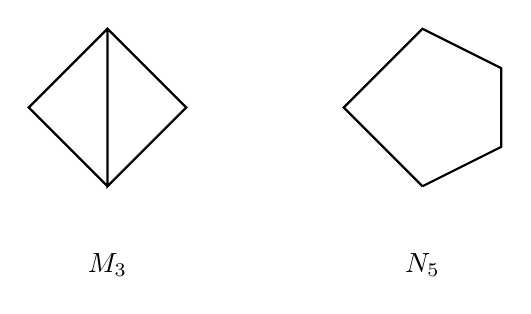
\begin{tikzpicture}
\po{(-2,0)}
\po{(-3,1)}
\po{(-2,1)}
\po{(-1,1)}
\po{(-2,2)}
\draw[thick] (-2,0) -- (-3,1) -- (-2,2) -- (-1,1) -- (-2,0) -- (-2,2);
\node at (-2,-1) {$M_3$};
\po{(2,0)}
\po{(1,1)}
\po{(3,.5)}
\po{(3,1.5)}
\po{(2,2)}
\node at (2,-1) {$N_5$};
\draw[thick] (2,0) -- (1,1) -- (2,2) -- (3,1.5) -- (3,.5) -- (2,0);
\end{tikzpicture}
\vspace{-5mm}
\end{center}
\caption{The lattices $M_3$ and $N_5$.}
\label{fig:nondist}
\end{figure}

\begin{proposition}\label{prop:distchar}
Let $L$ be a lattice. Then $L$ is distributive if, and only if, $L$ does not contain a sublattice which is isomorphic to $M_3$ or $N_5$.
\end{proposition}
Note that Proposition~\ref{prop:distchar} does not require the existence of a \emph{bounded} sublattice isomorphic to $M_3$ or $N_5$. %

\subsection*{Directed and filtering sets}
\label{def:directed} Let $P$ be a poset. A subset $D \subseteq P$ is called \emphind{directed} if it is non-empty, and for any $p, q \in D$, there exists $r \in D$ such that $r \geq p$ and $r \geq q$.
 Equivalently, $D$ is directed if any finite subset of $D$ has an upper bound in $D$ (Exercise~\ref{exe:directed}).  A \emphind{directed join} is the supremum of a directed set.
 Order-dually, a subset $F \subseteq P$ is called \emphind{filtering} if it is non-empty, and for any $p, q \in F$, there exists $r \in F$ such that $r \leq p$ and $r \leq q$.
 Again, equivalently, $F$ is filtering if any finite subset of $F$ has a lower bound in $F$.


In lattice theory, directed and filtering subsets of a lattice often appear, and indeed, certain filtering sets called \emph{prime filters} are central to the duality theory in Chapter~\ref{ch:priestley}, also see Exercise~\ref{exe:idealdirected}.  Directed and filtering sets are also important in topology and domain theory, as we will see in Chapters~\ref{chap:TopOrd},~\ref{chap:Omega-Pt}, and \ref{chap:DomThry}. In particular, we will often encounter the notion of a \emphind{filtering collection} of subsets of a set $X$, which is just a filtering subset of the poset $(\mathcal{P}(X), \subseteq)$. More explicitly, a non-empty collection $\mathcal{F}$ of subsets of a set $X$ is \emph{filtering} if, for any $S, T \in \mathcal{F}$, there exists $R \in \mathcal{F}$ such that $R \subseteq S \cap T$.

 
 A poset $P$ is \emph{directedly complete} \index{directedly complete poset} if any directed subset of $P$ has a supremum in $P$. Directedly complete posets are called \emphind{dcpo}'s, for short. Directed joins are what is needed to `complete' a lattice into a complete lattice, see Exercise~\ref{exe:directed}. A categorified version of this result will be proved in Proposition~\ref{prop:complete-category}.


\subsection*{Complements and Boolean algebras}
If $a$ is an element in a lattice, an element $b$ is called a \emph{complement} of $a$ if $a \wedge b = \bot$ and $a \vee b = \top$. A \emphind{Boolean algebra} is a distributive lattice in which each element has a complement. This complement is unique if it exists, see Exercise~\ref{exe:distuncomp}.a. If $L$ is a Boolean algebra, we denote by $\neg a$ the unique complement of an element $a$. 

The definition of Boolean algebras that we gave above was order-theoretic; there exist several equivalent \emph{equational} definitions. The simplest equational definition, and most useful for our purposes, is that a \emph{Boolean algebra} is a tuple $(B,\wedge,\vee,\bot,\top,\neg)$ such that $(B,\wedge,\vee,\bot,\top)$ is a distributive lattice, and for all $a \in B$, $a \wedge \neg a = \bot$ and $a \vee \neg a = \top$. The \emph{terminology} `Boolean algebra' comes from another (the original) equational definition: a Boolean algebra is the same thing as a commutative ring with unit in which all elements are idempotent, see Exercise~\ref{exe:BAeq} below.

Regarding maps between Boolean algebras, for any lattice homomorphism $f \colon L \to M$, where $L$ and $M$ are Boolean algebras, the function $f$ must also preserve the operation $\neg$, i.e., $f(\neg a) = \neg f(a)$ for all $a \in L$, see Exercise~\ref{exe:distuncomp}.b. We thus have an unambiguously defined notion of \emph{homomorphism} between Boolean algebras.\index{homomorphism!between Boolean algebras}

As a subclass of distributive lattices, Boolean algebras take up a very special position: every distributive lattice has a ``minimal'' Boolean algebra sitting around it, called its \emphind{Boolean envelope} or \emphind{free Boolean extension}\endnote{In some literature, this object is also called the \emphind{Booleanization}, but this term has also been used with other meanings, so we will avoid it.}. In categorical terms, Boolean algebras form a \emph{full reflective subcategory} of distributive lattices; see Chapter~\ref{ch:categories}. We end this section by defining what this means in elementary terms. 
\begin{definition}\label{def:booleanenvelope}
Let $L$ be a distributive lattice. A Boolean algebra $B$, together with an embedding $e \colon L \into B$, is called a \emphind{Boolean envelope} of $L$ if, for every lattice homomorphism $h \colon L \to A$, with $A$ a Boolean algebra, there exists a unique homomorphism $\bar{h} \colon A \to B$ such that $\bar{h} \circ e = h$, , i.e., such that the following diagram commutes:
\begin{center}
\begin{tikzpicture}
  \matrix (m) [matrix of math nodes,row sep=3em,column sep=3em,minimum width=3em]
  {
     B & A \\
     L &   \\
   };
  \path[-stealth]
    (m-1-1) edge node [above] {$\bar{h}$} (m-1-2)
    (m-2-1) edge node [left] {$e$} (m-1-1)
    (m-2-1) edge node [below] {$h$} (m-1-2);
\end{tikzpicture}
\end{center}
\end{definition}
In Proposition~\ref{prop:finite-boolenv} below, we will construct the Boolean envelope in the finite case, as a small application of the finite duality that we prove there. In fact, any distributive lattice has a Boolean envelope, and it is unique up to isomorphism; see Propositions~\ref{prop:boolenv-unique}~and~\ref{prop:boolenv} in Chapter~\ref{ch:priestley}.

\exercises
\begin{exercise}\label{exe:lattsuff}
Prove that, for a poset $(P,\leq)$ to be a lattice, it is sufficient that suprema and infima exist for the empty set and for all two-element subsets.
\end{exercise}
\begin{exercise}\label{exe:complattsuff}
Prove that, for a poset $(P,\leq)$ to be a complete lattice, it is sufficient that every subset has a supremum. By order-duality, it is also sufficient that every subset has an infimum.
\end{exercise}
\begin{exercise}
Let $L$ be a lattice. Prove that $\bot$ is an \emphind{identity element} for $\vee$, i.e., $a \vee \bot = a$ for all $a \in L$. By order-duality, $\top$ is an identity element for $\wedge$.
\end{exercise}
\begin{exercise}\label{exe:latticedefs}
\begin{enumerate}
\item Prove that the relation $\leq_L$ defined from a lattice according to the algebraic definition is a partial order in which all finite subsets have suprema and infima. \hint{Use the result of Exercise~\ref{exe:lattsuff}.}
\item Prove that, if $(L,\leq)$ is a lattice according to the order-theoretic definition, then $(L,\vee,\wedge,\bot,\top)$ is a lattice according to the algebraic definition, where the operations denote the binary and empty suprema and infima with respect to the partial order $\leq$.
\end{enumerate}
\end{exercise}
\begin{exercise}\label{exe:easy-counterexamples}
Find at least one example of each of the following:
\begin{enumerate}
\item a partial order which is not a total order;
\item a supremum which is not a maximum;
\item a poset in which finite joins exist but which is not a lattice;
\item a lattice which is not a complete lattice;
\item a subset of a lattice which is not a sublattice, even though it is a lattice in the inherited partial order;
\end{enumerate}
\end{exercise}
\begin{exercise}\label{exe:counterexamples-complete}
This exercise shows that there are some subtleties with the notion of completeness in lattices.
\begin{enumerate}

\item Prove that a complete lattice $L$ may contain a bounded sublattice $S$ which is also a complete lattice, but which contains a subset $E$ such that the supremum of $E$ in $S$ is different from the supremum of $E$ in $L$.

  \hint{Consider the sublattice of $\cP(\bN)$ that consists of $\bN$ itself and the finite sets of natural numbers.}
\item \label{ite:compDLnotframe} Show that a complete distributive lattice may fail to be a frame.
  
\hint{Use the same example as in the previous item.}
   
\end{enumerate}
\end{exercise}
\begin{exercise}\label{exe:injlatthom}
Let $f \colon L \to M$ be a function between lattices. Prove that
\begin{enumerate}
\item if $f$ is injective and preserves $\vee$ or $\wedge$, then $f$ is an order-embedding;
\item if $f$ is bijective and preserves $\vee$ or $\wedge$, then $f$ is a lattice isomorphism.
\end{enumerate}
\end{exercise}
\begin{exercise}\label{exe:disteq}
Let $L$ be a lattice. Prove that (\ref{eq:dist1}) and (\ref{eq:dist2}) are equivalent. \hint{You need to use the absorption laws twice.}
\end{exercise}
\begin{exercise}\label{exe:product-lattices}
Let $(L_i)_{i \in I}$ be an indexed family of lattices.
\begin{enumerate}
  \item Prove that $\prod_{i \in I} L_i$, as defined in the text, is indeed a lattice.
  \item Prove that the partial order on $\prod_{i \in I}L_i$ is given by the pointwise product of the partial orders on the $L_i$.
  \item Prove that $\prod_{i\in I}L_i$ is distributive if, and only if, $L_i$ is distributive for every $i \in I$.
\end{enumerate}
\end{exercise}
\begin{exercise}\label{exe:distchar}
Prove Proposition~\ref{prop:distchar}.
\end{exercise}

\begin{exercise}\label{exe:distuncomp}
\begin{enumerate}
\item Prove that, in a distributive lattice, any element has at most one complement.
\item\label{itm:lathomBA} Prove that any lattice homomorphism between Boolean algebras preserves the operation $\neg$.
\item Prove that any function between Boolean algebras that preserves $\neg$, $\bot$ and $\vee$ is a lattice homomorphism.
\end{enumerate}
\end{exercise}

\begin{exercise}\label{exe:directed}
\begin{enumerate}
\item   Let $P$ be a poset. Prove that, for any subset $D \subseteq P$, $D$ is directed if, and only if, any finite subset of $D$ has an upper bound in $D$. (Note that the empty set is always a subset of $D$, and that any element of $D$ will be an upper bound for it.)
\item Let $L$ be a bounded lattice. Prove that $L$ is a complete lattice if, and only if, $L$ is a dcpo.
\item Give an example of a dcpo that is not a lattice.
\end{enumerate}
\end{exercise}

\begin{exercise}\label{exe:BAeq}
Let $(B,+,\cdot,0,1)$ be a commutative ring with unit in which $a^2 = a$ for all $a \in B$. Define $a \leq b$ if, and only if, $a \cdot b = a$. Prove that $\leq$ is a distributive lattice order on $B$, and that
 every element of $B$ has a complement with respect to $\leq$. \emph{Hint:} first show that $a + a = 0$ for all $a \in B$.

Conversely, let $(B,\wedge,\vee,\bot,\top,\neg)$ be a Boolean algebra. Define, for any $a, b \in B$, $a + b := (a \wedge \neg b) \vee (\neg a \wedge b)$, $a \cdot b := a \wedge b$, $0 := \bot$ and $1 := \top$. Prove that $(B,+,\cdot,0,1)$ is a commutative ring with unit in which $a^2 = a$ for all $a \in B$.
\end{exercise}

\begin{exercise}\label{exe:adjointexistsiff}
This exercise guides you through a proof of the `\emphind{adjoint functor theorem for complete lattices}'. Let $C, D$ be complete lattices and $f \colon C \to D$ a function.
\begin{enumerate}
\item Suppose that $f$ preserves arbitrary suprema. For each $d \in D$, define $g(d) := \bigvee \{c \in C \ | \ f(c) \leq d\}$. Prove that $g$ is upper adjoint to $f$.
\item Conclude from the previous item and Exercise~\ref{exe:adjunctions}.\ref{itm:leftadjointpreservessup} that a function $f$ between complete lattices possesses an upper adjoint if, and only if, $f$ preserves arbitrary suprema.
\item Conclude from the previous item, applied to $C^\op$ and $D^\op$, that a function $f$ between complete lattices possesses a lower adjoint if, and only if, $f$ preserves arbitrary infima.
\end{enumerate}
\end{exercise}
\begin{exercise}\label{exe:adjointsfix}
  Let $f \colon C \leftrightarrows D \colon g$ be an adjunction between complete lattices, with $f$ left adjoint to $g$.
  \begin{enumerate}
  \item Show that the image of $g$ in $C$ is closed under arbitrary meets.
  \item Show that the image of $g$ is isomorphic to the image of $f$ in $D$.
  \item Give an example showing that the image of $g$, despite being a complete lattice in its own right, need not be a sublattice of $C$.
 \end{enumerate}
\end{exercise}

\begin{exercise}\label{exe:congruencelattice}
\begin{enumerate}
  \item Prove that the collection of congruences on a lattice $L$ is a complete lattice under the inclusion order.
  \item Prove that this lattice of congruences is always distributive, even if $L$ is not.
\end{enumerate}
\end{exercise}

\section{Duality for finite distributive lattices}\label{sec:finDLduality}
Lattices were introduced as abstract structures in the previous section. In this section we show that finite distributive lattices can be represented in a more concrete way, namely, as certain collections of subsets of a given set.\endnote{The results in this section are essentially due to Birkhoff \cite{Bir1933} and are also consequences of the more general results of Stone \cite{Sto1937/38}, which we will present later in this text.} %
This representation gives rise to our first example of a \emph{duality}. From it, we also immediately deduce a duality for finite Boolean algebras.\endnote{\label{not:nondistcase1}There exist similar, but more involved results for (finite) lattices that are not necessarily distributive. In this text, however, we will limit ourselves to distributive lattices. More information and references on general lattices can be found, e.g., in \cite{DavPri2002} and also in the introduction of our paper \cite{GehGoo2014}.}

For any set $S$, we denote by $\mathcal{P}(S)$\nomenclature[power set]{\mathcal{P}(-)}{power set} the \emphind{power set} of $S$, that is, the collection of all subsets of $S$. The \emphind{inclusion order} of subsets gives a partial order on $\mathcal{P}(S)$, which is in fact a distributive lattice. (Indeed, $\mathcal{P}(S)$ is even a \emph{Boolean algebra}.) Any sublattice of $\mathcal{P}(S)$ is a distributive lattice, too. Conversely, any distributive lattice is a sublattice of a power set lattice, as we will see in Chapter 3. %
In this section, we will prove a stronger result for \emph{finite} distributive lattices (Proposition~\ref{prop:birkhoff}).

Let $(P,\preceq)$ be a preorder. An \emphind{up-set} is a subset $U \subseteq P$ such that whenever $p \in U$ and $p \preceq q$, we have $q \in U$. A \emphind{down-set} is a subset $D \subseteq P$ such that whenever $p \in D$ and $q \preceq p$, we have $q \in D$. For $p \in P$, the \emphind{principal up-set} generated by $p$, ${\uparrow} p$, is the set of elements above $p$, and the \emph{principal down-set} generated by $p$, ${\downarrow} p$, is the set of elements below $p$. By a \emphind{convex set} we mean a set that is an intersection of an up-set and a down-set, also see Exercise~\ref{ex:convex}.

The preorder $\preceq$ specifies two sublattices of $\mathcal{P}(P)$, namely, the sublattice $\Up(P,\preceq)$ of \emph{up-sets} with respect to $\preceq$, and the sublattice $\Down(P, \preceq)$ of \emph{down-sets} with respect to $\preceq$. (Exercise~\ref{exe:updownsublat} asks the reader to verify that these are indeed sublattices.) Notice that, if $U$ is an up-set, then its complement, $P \setminus U$, is a down-set, and vice versa; therefore, $\Up(P,\preceq)$ is isomorphic to $\Down(P,\preceq)^\op$, or, said otherwise, $\Up(P,\preceq)$ and $\Down(P,\preceq)$ are \emph{dually isomorphic}. 

\begin{notation}
  Throughout this book, when $U$ is a subset of a set $P$, we often use the notation $U^c$ instead of $P \setminus U$ for the \emphind{complement} of a subset $U$. Note that this abbreviated notation $U^c$ assumes that the `ambient' set $P$ is clear from the context.
\end{notation}

Let $j$ be an element of a lattice $L$. Then $j$ is called (finitely) \emphind{join-irreducible} if, whenever $j = \bigvee S$ for a finite $S \subseteq L$, we have $j \in S$. Notice that $\bot$ is never a join-irreducible element, because $\bot = \bigvee \emptyset$.
We denote by $\J(L)$ the poset of join-irreducible elements of $L$, where the order is the restriction of the order on $L$.
Similarly, $m \in L$ is (finitely) \emphind{meet-irreducible} if $m = \bigwedge S$ implies $m \in S$ for any finite $S \subseteq L$, $\top$ is never meet-irreducible, and $\M(L)$ denotes the poset of meet-irreducible elements of $L$.

An important and useful fact about \emph{finite} lattices is that there are `enough' join-irreducibles to separate elements, in the following sense.\index{enough join-irreducibles}
\begin{lemma}\label{lem:finiteperfect}
Let $L$ be a finite lattice. For any $a, b \in L$, if $a \nleq b$, then there exists $j \in \J(L)$ such that $j \leq a$ and $j \nleq b$.
\end{lemma}
\begin{proof}
The set $T := ({\downarrow} a) \setminus ({\downarrow} b)$ of elements that are below $a$ but not below $b$ is non-empty, as it contains $a$. Since $L$ is finite, pick a minimal element $j$ of $T$. This element $j$ must be join-irreducible. Indeed, suppose that $j = \bigvee S$ for some finite $S \subseteq L$. Then, since $\bigvee S \nleq b$, pick $c \in S$ such that $c \nleq b$. Since $c \leq j \leq a$, we have $c \in T$, so the minimality of $j$ implies that $j = c$.
\end{proof}

For any finite lattice $L$, consider the function
\begin{align*}
\widehat{(-)} \colon &L \to \Down(\J(L)) \\
			&a \mapsto \widehat{a} := \{j \in \J(L) \ | \ j \leq_L a\},
\end{align*}
which sends every element of the lattice to the down-set of join-irreducibles below it. This function $\widehat{(-)}$ is obviously order-preserving, and Lemma~\ref{lem:finiteperfect} says precisely that $\widehat{(-)}$ is an order-embedding. When is $\widehat{(-)}$ surjective, and hence an order isomorphism? We give the answer in the next proposition.

An element $j$ in a lattice $L$ is \emph{join-prime} if, for every finite $S \subseteq L$, $j \leq \bigvee S$ implies $j \leq a$ for some $a \in S$. Note that any join-prime element in a lattice is in particular join-irreducible. \emph{Meet-prime} elements are defined in an order-dual way.
\begin{proposition}\label{prop:birkhoff}
Let $L$ be a finite lattice. The following are equivalent:
\begin{enumerate}
\item[(i)] the lattice $L$ is distributive;
\item[(ii)] every join-irreducible element of $L$ is join-prime;
\item[(iii)] the function $\widehat{(-)}$ is an order-isomorphism.
\end{enumerate}
\end{proposition}
\begin{proof}
(i) $\Rightarrow$ (ii). Let $j$ be join-irreducible. If $j \leq \bigvee S$ for some finite $S$, then
\[ j = j \wedge \left( \bigvee S \right) = \bigvee_{a \in S} (j \wedge a),\]
where we use the distributive law in the last step. Since $j$ is join-irreducible, $j = j \wedge a$ for some $a \in S$, which means that $j \leq a$.

(ii) $\Rightarrow$ (iii). If $D \in \Down(\J(L))$ and $j \in \J(L)$, then $j \leq \bigvee D$ if, and only if, $j \in D$. Thus, $\widehat{\bigvee D} = D$, showing that $\widehat{(-)}$ is surjective.

(iii) $\Rightarrow$ (i) is clear, because $\Down(\J(L))$ is distributive.
\end{proof}
Note that the proof of implication (i) $\Rightarrow$ (i) in Proposition~\ref{prop:birkhoff} did not use the assumption that $L$ is finite. Therefore, this proposition also implies that in any distributive lattice $L$, \emph{join-prime} and \emph{join-irreducible} are synonymous.


If $L$ is a finite distributive lattice, we call $\J(L)$ the \emphind{dual poset} of $L$. If $P$ is a finite poset, we call $\Down(P)$ the \emphind{dual distributive lattice} of $P$. With this terminology, Proposition~\ref{prop:birkhoff} implies that any finite distributive lattice is isomorphic to its double dual.
To turn this representation result into a \emph{duality}, we now consider maps. If $f \colon P \to Q$ is an order-preserving function between preorders, then the \emphind{inverse image} map
\begin{align*}
\Down(f) \colon &\Down(Q) \to \Down(P) \\
&D \mapsto f^{-1}(D)
\end{align*}
is a lattice homomorphism.  We will prove in Proposition~\ref{prop:finDLmorphisms} below that, in the special case where $P$ and $Q$ are finite posets, every lattice homomorphism $\Down(Q) \to \Down(P)$ arises in this way. Before we can do so, we need a general lemma about adjunctions between finite lattices.
\begin{lemma}\label{lem:loweradj-preserves-joinprime}
Let $g \colon D \leftrightarrows E \colon h$ be an adjunction between finite lattices, and further suppose that $h$ preserves suprema. Then, for any join-prime element $j$ in $D$, the element $g(j)$ is join-prime in $E$.
\end{lemma}
\begin{proof}
Let $S \subseteq E$ be an arbitrary subset such that $g(j) \leq \bigvee S$. Then, since $h$ is upper adjoint to $g$, $j \leq h(\bigvee S) = \bigvee h(S)$, where we use that $h$ preserves suprema. Since $j$ is join-prime, pick $s \in S$ such that $j \leq h(s)$. Since $g$ is lower adjoint to $h$, $g(j) \leq s$. Thus, $g(j)$ is join-prime.
\end{proof}
\begin{proposition}\label{prop:finDLmorphisms}
Let $P$ and $Q$ be finite posets. For any lattice homomorphism $h \colon \Down(Q) \to \Down(P)$, there exists a unique order-preserving $f \colon P \to Q$ such that $h = \Down(f)$.
\end{proposition}
\begin{proof}
Since $h$ preserves all infima, it has a lower adjoint, $g$, by Exercise~\ref{exe:adjointexistsiff}(c). By Lemma~\ref{lem:loweradj-preserves-joinprime}, since $h$ also preserves all suprema, $g$ sends join-prime elements to join-prime elements. Now, if $p \in P$, then ${\downarrow}p$ is join-prime (Exercise~\ref{exe:irrindownset}), and thus $g({\downarrow}p)$ is join-prime. Again by Exercise~\ref{exe:irrindownset}, pick the unique $f(p) \in Q$ such that $g({\downarrow}p) = {\downarrow}f(p)$.
Notice that the function $f \colon P \to Q$ thus defined is order-preserving, because $g$ is order-preserving, so $p \leq p'$ implies $f(p) \in {\downarrow} f(p) = g({\downarrow} p) \subseteq g({\downarrow} p') = {\downarrow} f(p')$.

Moreover, for any $E \in \Down(Q)$ and $p \in P$, we have, using the adjunction and the definition of $f$, that
\[p \in h(E) \iff {\downarrow} p \subseteq h(E) \iff g({\downarrow}p) \subseteq E \iff {\downarrow} f(p) \subseteq E \iff f(p) \in E,\]
so that $h(E) = f^{-1}(E)$, as required.
The uniqueness of $f$ is left as Exercise~\ref{exe:completeuniquenesspart}.
\end{proof}


Summing up, we have associated to every finite distributive lattice $L$ a finite poset $\J(L)$, that we called the dual poset of $L$, and, conversely, to every finite poset $P$, a finite distributive lattice $\Down(P)$ that we called the dual distributive lattice of $P$. We have proved that:
\begin{enumerate}
\item[(1)] every finite distributive lattice is isomorphic to its double dual (Proposition~\ref{prop:birkhoff}),
\item[(2)] homomorphisms between finite distributive lattices are in one-to-one correspondence with order-preserving functions between their dual posets (Proposition~\ref{prop:finDLmorphisms}).
\end{enumerate}
The reversal of direction of arrows when moving to `the other side', i.e., a function from $P$ to $Q$ gives a function from $\Down(Q)$ to $\Down(P)$, is what makes the correspondence in (2) `\emph{dual}'. What all this means, in practice, is that finite distributive lattices with homomorphisms between them are \emph{essentially the same thing} as finite posets with order-preserving functions between them.

In fancier terms, we have proved the following theorem.  \index{duality!for finite distributive lattices} \index{Birkhoff duality} \index{duality!Birkhoff}
\begin{theorem}\label{thm:birkhoffduality}
The functors $\Down$ and $\J$ constitute a duality between the category $\DL_f$ of finite distributive lattices with homomorphisms and the category $\Pos_f$ of finite posets with order-preserving functions.
\end{theorem}
We will define the precise meaning of the terms (`category', `functor', `duality') used in this theorem in Section~\ref{sec:external} in Chapter~\ref{ch:categories},
but the reader who is not yet familiar with these terms can rest assured that the mathematical content of the theorem consists precisely of items (1) and (2) above. For a precise explanation of why what we have proved here shows that the functors form a duality, see Example~\ref{exa:cat-duality-examples} on p.~\pageref{exa:cat-duality-examples}.\\

\subsection*{Duality for finite Boolean algebras}
We end this section by describing how Theorem~\ref{thm:birkhoffduality} specializes to finite Boolean algebras.
An \emphind{atom} of a lattice $L$ is a minimal non-bottom element, i.e., an element $j \in L$ such that $j \neq \bot$ and $\bot \leq a \leq j$ implies $a = \bot$ or $a = j$ for any $a \in L$.
\begin{proposition}\label{prop:birkhoffBA}
Let $L$ be a finite distributive lattice. The following are equivalent:
\begin{enumerate}
\item[(i)] the distributive lattice $L$ is a Boolean algebra;
\item[(ii)] every join-irreducible element of $L$ is an atom;
\item[(iii)] the order on $\J(L)$ is trivial, i.e., distinct elements are incomparable;
\item[(iv)] the distributive lattice $L$ is isomorphic to $\mathcal{P}(\J(L))$.
\end{enumerate}
\end{proposition}
\begin{proof}
(i) $\Rightarrow$ (ii). Let $j \in \J(L)$. Suppose that $\bot \leq a \leq j$. Since $a \vee \neg a = \top$, we have $j \leq a \vee \neg a$. Since $L$ is distributive, by Proposition~\ref{prop:birkhoff} $j$ is join-prime, so $j \leq a$ or $j \leq \neg a$. If $j \leq a$, then $a = j$, and we are done. If $j \leq \neg a$, then $a \leq j \leq \neg a$, so $a = a \wedge \neg a = \bot$.

(ii) $\Rightarrow$ (iii). Clear from the definition of atom.

(iii) $\Rightarrow$ (iv). By Proposition~\ref{prop:birkhoff}, $L$ is isomorphic to $\Down(\J(L))$. By (3), any subset of $\J(L)$ is a down-set.

(iv) $\Rightarrow$ (i). Clear because $\mathcal{P}(\J(L))$ is a Boolean algebra.
\end{proof}
Proposition~\ref{prop:birkhoffBA} shows in particular that every finite Boolean algebra $L$ is of the form $\mathcal{P}(S)$, where $S$ is the finite set of atoms (= join-irreducibles) of $L$.

Note also from (3) in Proposition~\ref{prop:birkhoffBA} that, if $L$ is a finite Boolean algebra and $M$ is a finite distributive lattice, then \emph{any} function $f \colon \J(L) \to \J(M)$ is order-preserving. Thus, the lattice homomorphisms $M \to L$ are exactly the inverse images of functions $\J(L) \to \J(M)$. In particular, if both $L$ and $M$ are both finite Boolean algebras, then homomorphisms from $L$ to $M$ correspond to functions $\J(M) \to \J(L)$. We conclude:\index{duality!for finite Boolean algebras} \index{Birkhoff duality} \index{Stone duality!finite case}
\begin{theorem}\label{thm:birkhoffdualityBA}
The functors $\mathcal{P}$ and $\J$ constitute a duality between the category $\BA_f$ of finite Boolean algebras with homomorphisms and the category $\Set_f$ of finite sets with functions.
\end{theorem}

As promised at the end of the previous section, we end this first chapter by using the dualities to give a simple concrete description of the \emphind{Boolean envelope} of a distributive lattice, defined in the previous section.
\begin{proposition}\label{prop:finite-boolenv}
  Let $L$ be a finite distributive lattice. Then the finite Boolean algebra $L^- := \mathcal{P}(\mathcal{J}(L))$, with the embedding $\widehat{(-)} \colon L \to L^-$, is a Boolean envelope of $L$.
  \end{proposition}
  \begin{proof}
  Let $h \colon L \to A$ be a lattice homomorphism, with $A$ a Boolean algebra. By the results in this section, we may assume, up to isomorphism, that $L = \mathcal{D}(P)$ for a poset $P$, $A = \mathcal{P}(X)$ for a set $X$, and $h = f^{-1}$ for a function $f \colon X \to P$. The function $\bar{h}$, defined by sending any $u \in \mathcal{P}(P)$ to $f^{-1}(u)$, is clearly a homomorphism extending $h$. The uniqueness is left as Exercise~\ref{ex:unique-finite-boolean-envelope}; or see the more general proof of Proposition~\ref{prop:boolenv} in Chapter~\ref{ch:priestley}.
  \end{proof}


This intimate connection between distributive lattices and Boolean algebras, and the various dualities for them, will be made more precise in Section~\ref{sec:topologize} in Chapter~\ref{ch:priestley}, and further in Section~\ref{sec:StoneSpaces} in Chapter~\ref{chap:Omega-Pt}.

\exercises
\begin{exercise}\label{exe:updownsublat}
Let $P$ be a poset. Prove that $\Down(P)$ is a sublattice of $\Po(P)$. Use order-duality to deduce that $\Up(P)$ is also a sublattice of $\Po(P)$.
\end{exercise}

\begin{exercise}\label{ex:convex}
Prove that a subset $C$ of $P$ is convex if, and only if, for any $p, q \in C$, if $p \leq r \leq q$, then $r \in C$.
\end{exercise}

\begin{exercise}\label{exe:joinirralt}
Prove that an element $j$ in a lattice $L$ is join-irreducible if, and only if, $j \neq \bot$ and for any $x,y \in L$, if $j = x \vee y$, then $j = x$ or $j = y$.
\end{exercise}


\begin{exercise}\label{exe:perfect}
\begin{enumerate}
\item Formulate a lemma which says that any finite lattice has enough meet-irreducibles, and prove it (you may use Lemma~\ref{lem:finiteperfect}).
\item Give an example of a lattice which does not have enough join-irreducibles.
\item Give an example of a complete lattice which has enough join-irreducibles, but not enough meet-irreducibles.
\item Can you find an example as in (c) with the additional requirement that the complete lattice is a \emph{frame}? That it is a \emph{Boolean algebra}? If not, formulate and prove a result about this.
\end{enumerate}
\end{exercise}

\begin{exercise}\label{exe:joinirrjoinp}
\begin{enumerate}
\item Prove that any join-prime element in a lattice is join-irreducible.
\item Give an example of a lattice and a join-irreducible element in it that is not join-prime.
\end{enumerate}
\end{exercise}


\begin{exercise}\label{exe:irrindownset}
Let $P$ be a finite poset and $D \in \Down(P)$. Prove that:
\begin{enumerate}
\item $D$ is join-irreducible if, and only if, $D$ is a principal down-set, i.e., $D = {\downarrow} p$ for some $p \in P$.
\item $D$ is meet-irreducible if, and only if, $D$ is the complement of a principal up-set, i.e,. $D = P \setminus ({\uparrow} p)$ for some $p \in P$.
\end{enumerate}
Conclude from the first part of this exercise that $\J(\Down(P))$ is a poset isomorphic to $P$.
\end{exercise}

\begin{exercise}\label{exe:completeuniquenesspart}
Complete the uniqueness part of the proof of Proposition~\ref{prop:finDLmorphisms} by showing that, if $f, f' \colon P \to Q$ are order-preserving and $\Down(f) = \Down(f')$, then $f = f'$.%
\end{exercise}

\begin{exercise}\label{exe:kappa}
Let $L$ be a finite distributive lattice.
\begin{enumerate}
\item Prove that, for any $j \in \J(L)$, the set
\[ L \setminus ({\uparrow} j) = \{a \in L \ | \ j \nleq a\}\]
has a maximum. We denote this maximum by $\kappa(j)$.
\item Prove that, for any $j \in \J(L)$ and $a \in L$, $j \nleq a$ if, and only if, $a \leq \kappa(j)$.
\item Prove that $\kappa(j)$ is meet-irreducible for any $j \in \J(L)$.
\item Prove that $\kappa \colon \J(L) \to \M(L)$ is an order-isomorphism.
\end{enumerate}
\end{exercise}

\begin{exercise}\label{ex:unique-finite-boolean-envelope}
Prove that the function $\bar{h}$ defined in the proof of Proposition~\ref{prop:finite-boolenv} is unique. \hint{It suffices (why?) to prove that the sublattices $\mathcal{D}(P)$ and $\mathcal{U}(P)$ together generate $\mathcal{P}(P)$. For this, note first that any singleton $\{p\}$ can be obtained as the intersection of the down-set ${\downarrow} p$ and the up-set ${\uparrow} p$; then use that any $u \in \mathcal{P}(P)$ can be written as a (finite) union of singletons.}
\end{exercise}

\theendnotes
\setcounter{endnote}{0}


